\section{Results}
\label{sec:results}

\subsection{Sampling error is set by design leverage (H1)}
With a correctly specified linear one-hop response, the RMSE of \textsc{ols-s} grows with mean degree with log-log slope $0.52$ in $\log(1+d)$ (ER) and falls with $n$ with slope $-0.50$ (Fig.~\ref{fig:var}a--b), as Prop.~\ref{prop:lev} implies. DiM does not improve with $n$ (its error is bias); H\'ajek is defined in more than half of the draws only for $n\ge8000$ at $d=16$ and has RMSE $1.3$--$1.4$ there. With one constant $\hat\kappa=1.09$ fitted on the 72 ER/Bernoulli runs, $\hat\kappa\sqrt{L/n}$ matches the observed RMSE of all 162 Bernoulli-design runs with median ratio $1.01$ and range $[0.85,1.13]$ ($98\%$ within $\pm10\%$; Fig.~\ref{fig:var}c), including the 90 non-ER runs (SBM, WS, BA, Stanford3, ego-Facebook) never used for fitting; simulated leverage equals the formula within $7\%$ for Bernoulli designs (App.~\ref{app:extra}).

\textbf{Cluster randomization lowers leverage; the closed form is rougher there.} With $\approx30$--$40$ clusters RMSE falls from $0.22$ to $0.04$ ($5\times$) on WS ($d{=}40$), from $0.120$ to $0.042$ ($2.9\times$; leverage $48.9\to5.6$) on ego-Facebook and from $0.071$ to $0.037$ ($1.9\times$; $47.1\to14.6$) on Stanford3, but only $1.2$--$1.6\times$ on SBM and $1.0$--$1.3\times$ on BA, whose clusterings cut $57\%$--$87\%$ of the edges. For the 126 cluster-design runs the formula underpredicts RMSE in $73\%$ (median ratio $1.10$, IQR $[1.00,1.29]$, range $[0.69,3.74]$); extremes occur with $\le10$ clusters, where one draw's sample covariance of $(z,s)$ differs from its expectation. Rank correlation between $\sqrt{L/n}$ and RMSE over all 288 runs is $0.96$.

\begin{figure}[t]
\centering
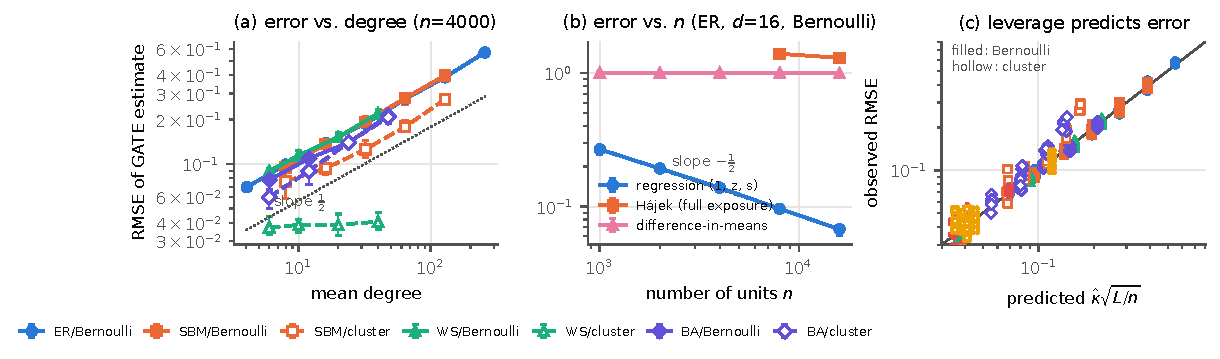
\includegraphics[width=\linewidth]{figs/fig_variance.pdf}
\caption{Variance side (E1). (a) RMSE of \textsc{ols-s} vs mean degree for five graph families under Bernoulli (solid) and cluster randomization (dashed, $K{=}40$ target clusters); dotted: slope $\frac12$. (b) RMSE vs $n$ on ER graphs with $d{=}16$: regression, H\'ajek (shown only where defined in $>50\%$ of assignments) and DiM. (c) Observed RMSE vs $\hat\kappa\sqrt{L/n}$ (closed-form leverage; one global $\hat\kappa$ fitted on ER/Bernoulli runs) for 288 runs including Stanford3 and ego-Facebook. Markers: mean over 6 worlds; bars: min--max over worlds (panels a--b); panel c shows each setting-world pair mean.}
\label{fig:var}
\end{figure}

\subsection{Extrapolation bias under nonlinear response does not vanish with $n$ (H2)}
Prop.~\ref{prop:extrap} gives the bias of the linear one-hop regression for any response shape from exact binomial moments. Over 63 (graph, shape, degree, $n$) Bernoulli settings the simulated bias differs from it by at most $0.012$ (median $0.003$) on a GATE of $\approx2$ (Fig.~\ref{fig:ext}a). It depends on the tangent slope at $p$: on ER ($d{=}30$) it is $\approx0$ for $k=2$, $-0.45$ for $k=4$, $-0.28$ for $k=\frac12$ and $+1.47$ for the threshold response (Appendix Table~\ref{tab:extrap}); it grows with degree as exposures concentrate near $p$ (Fig.~\ref{fig:ext}b) and is unchanged from $n=10^3$ to $1.6\times10^4$ (c). Combining the closed-form bias and leverage, $\sqrt{B^2+\hat\kappa^2L/n}$ matches the observed RMSE with median ratio $1.005$ (IQR $[0.99,1.03]$; $89\%$ within $\pm10\%$) over 360 world-settings (d).

\textbf{Flexible regressions help only where the graph provides extreme exposures.} Under Bernoulli($\frac12$) the share of units with $s\le0.1$ or $s\ge0.9$ is $0.0\%$ on ER/regular graphs ($d{=}30$), $0.5\%$ on BA, $6.5\%$ on Stanford3 and $4.3\%$ on ego-Facebook (and $79\%$ on ego-Facebook under cluster randomization). Where such units exist, a cubic in $s$ removes nearly all bias for every shape (Stanford3: $|$bias$|\le0.03$, RMSE $0.08$--$0.09$ vs $0.07$ for the linear model under a linear response; ego-Facebook: $|$bias$|\le0.07$, RMSE $0.17$--$0.18$ vs $0.12$), costing $15$--$45\%$ RMSE when the linear model was right. On ER the cubic has RMSE $1.9$--$3.1$ for all shapes and the quadratic leaves the bias unchanged (threshold: $1.47\to1.47$). Gradient boosting on $(z,s,s^{(2)},\ell)$ cannot extrapolate: even for a \emph{linear} response it is biased towards DiM ($-0.52$ on ER, $-0.24$ on Stanford3, $-0.13$ on ego-Facebook), but it has the lowest RMSE when the response is steep and the linear model badly wrong (threshold, Bernoulli: $0.52$ vs $1.47$ on ER, $0.26$ vs $0.38$ on Stanford3, $0.41$ vs $0.61$ on ego-Facebook) and is much worse when the linear model is adequate ($0.74$ vs $0.17$ on ER; 3 worlds, 40 assignments). Cluster randomization shrinks the linear model's bias where clusters are good (ego-Facebook $k{=}4$: $-0.22\to-0.03$; threshold $0.60\to0.05$) and little elsewhere (ER $k{=}4$: $-0.45\to-0.36$; Stanford3: $-0.13\to-0.12$).

\begin{figure}[t]
\centering
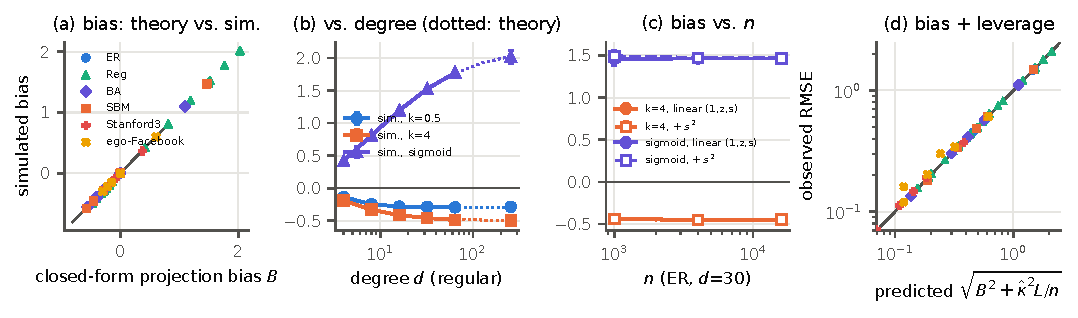
\includegraphics[width=\linewidth]{figs/fig_extrap.pdf}
\caption{Extrapolation bias (E2). (a) Simulated bias of \textsc{ols-s} vs the closed-form bias of Prop.~\ref{prop:extrap}, 63 Bernoulli settings (mean over 6 worlds). (b) Bias vs degree on random regular graphs ($n{=}4000$): simulation (solid; bars min--max) and theory (dotted). (c) Bias vs $n$, $k{=}4$ and threshold response, linear and $+s^2$ regressions. (d) Observed RMSE vs $\sqrt{B^2+\hat\kappa^2L/n}$ (closed-form $B$ and $L$, $\hat\kappa$ from E1).}
\label{fig:ext}
\end{figure}

